\documentclass[a4paper,review,12pt,authoryear]{elsarticle}

% \usepackage{natbib}
\usepackage{amsfonts,amsmath,bbm,bm,xcolor,booktabs,hyperref,amsthm}
\usepackage{geometry}
\usepackage{subfig}
\geometry{a4paper,scale=0.8}
\usepackage{setspace}
\setstretch{1.5}
\let\code=\texttt
\let\proglang=\textsf
\setcounter{MaxMatrixCols}{20}

\hypersetup{
  colorlinks=true,
  linkcolor=blue,
  citecolor=blue,
  urlcolor=blue}

% ADDING LINENUMBERS FOR REVIEWING:
% \usepackage{lineno}

\begin{document}

\begin{frontmatter}

  \title{Constructing hierarchies}


  \begin{abstract}

    

  \end{abstract}

  \begin{keyword}
  Forecasting \sep
  Hierarchical time series \sep
  
  \end{keyword}

\end{frontmatter}

%\clearpage
\newpage
% \linenumbers

\section{Introduction}


\section{Methodology}
\label{sec:method}

\subsection{Framework}

1. construct hierarchies based on historic observations
2. forecast and reconciliation
3. evaluation

\subsection{Constructing hierarchies by clustering}

\cite{aghabozorgiTimeseriesClusteringDecade2015a} summarised the four components of time series clustering, including time series representations, distance measures, clustering algorithms and evaluation. In our framework, the first three components are involved in the constructing hierarchies procedure. The last component includes evaluation of reconciled forecasts of the original hierarchy.

\subsubsection*{Time series representations}

Time-series representations represent raw time series in another space through techniques like feature extraction or dimensionality reduction. By utilising diverse time series representations, we are able to obtain distinct clusters which offer varied perspectives on the same dataset. 
Despite the absence of the theoretical evidence regarding how groups in hierarchical time series affect forecast reconciliation performance, we seek to explore multiple time series representations and discern potential correlations between hierarchical structure and the efficacy of forecast reconciliation.

Considering the impracticality of exploring every conceivable time series representation, we focus on four key ones: raw time series, in-sample error, features of time series, and features of in-sample error.
The inclusion of raw time series is motivated by its simplicity and broad applicability.
A crucial element contributing to the success of the minimum trace method proposed by \cite{wickramasuriyaOptimalForecastReconciliation2019} lies in estimating the covariance matrix of base forecast errors based on in-sample fit error. Hence, we consider in-sample error as a representation to examine how the structure within the error series influences reconciliation performance. Notably, to the best of our knowledge, we are the first to utilise in-sample error as a time series representation in the context of forecast reconciliation literature.
The time series and in-sample error representations are standardised on a per-series basis to eliminate the impact of scale variations.
Features, widely employed in capturing time series characteristics across literature, play a pivotal role in various time series applications, including clustering (\citealp{tianoFeatTSFeaturebasedTime2021}) and forecasting (\citealp{wangUncertaintyEstimationFeaturebased2022, liFeaturebasedIntermittentDemand2023}). In our exploration, we incorporate features of both time series and in-sample fit error as representations. These representations allow us to glean insights into the diverse aspects of hierarchical time series data and enhance our understanding of how different structures contribute to the forecast reconciliation performance.


 


\subsubsection*{Distance measures}

Distance measures serve as crucial tools for assessing the similarity between two series, forming the foundation for clustering algorithms to detect clusters within datasets. In the realm of time series clustering literature, we consider two widely applied distance measures: Euclidean distance and dynamic time warping (DTW) (\citealp{warrenliaoClusteringTimeSeries2005}). 

Given the limited number of time series in comparison to the variable dimensions (i.e., the length of time series and the number of time series features) within hierarchical time series in our applications, dimension reduction on the aforementioned representations becomes imperative when employing Euclidean distance. Failure to undertake dimension reduction may result in undesirable clustering outcomes due to the challenges posed by the curse of dimensionality. To address this, we perform principal component analysis, extracting the first few principal components that collectively explain at least 80\% of the variance within the data.

In contrast, DTW (\citealp{sakoeDynamicProgrammingAlgorithm1978}), demonstrates reduced sensitivity to the curse of dimensionality. Unlike the one-to-one point comparison inherent in Euclidean distance, DTW accommodates time series of varying lengths through many-to-one comparisons. This adaptive approach allows for the recognition of time series with similar shapes, even in the presence of signal transformations such as shifting and/or scaling.


\subsubsection*{Clustering algorithms}
\label{sec:clustering}

Regarding clustering algorithms, we consider two common approaches, k-Medoids and agglomerative hierarchical clustering. K-Medoids algorithm is one of the classical partitioning clustering algorithms. The idea behind partitioning clustering is the minimisation of the total distance between all samples in a cluster from their cluster centres.  We consider k-Medoids instead of the well known k-Means because k-Means use mean vector of samples within a cluster as cluster centre, which is not trivial when using DTW distance measure. In contrast, k-Medoids select one of the samples in the cluster as cluster centre. We use the k-Meodoids variants partitioning around medoids (PAM, \citealp{PartitioningMedoidsProgram1990}). The most important parameter for k-Medoids algorithm is the number of cluster. We follow the suggestion of \cite{PartitioningMedoidsProgram1990} to choose the optimal number of cluster by average silhouette width (ASW), which is a popular cluster validation index to estimate the number of clusters. Given a clustering $\mathcal{C}$, the silhouette width for the $i$th sample is calculated as 
\[
  SW(i) = \frac{b(i)-a(i)}{\max\{a(i), b(i)\}},  
\]
where $a(i)$ is the average distance of $i$the sample to samples in the cluster to which it is assigned, and $b(i)$ is the average distance of $i$th sample to the samples in the nearest cluster it is not assigned. A large value of silhouette means that the corresponding sample is much closer to the samples to the samples in its own cluster than to the neighbouring one. Silhouette width is zero for the sample which is the only sample in its cluster. ASW is calculated as the average of silhouette widths of all samples. By iterating over all possible number of clusters, we choose the clustering result $\mathcal{C}$ that maximises the ASW as the optimal result. One drawback of this approach is that ASW does not exist when there is only one cluster, meaning that it can not determine whether there are well separated clusters or not. Gap statistics (\citealp{tibshiraniEstimatingNumberClusters2002}) can address this issue, but it can not be used with DTW.

hierarchical clustering

\subsection{Constructing hierarchies randomly}

pure random

random based on specific structure

\subsection{Forecast combination}

\section{Simulation}
\label{sec:simulation}

In this section, we demonstrate that hierarchies constructed by clustering may not outperform hierarchies constructed randomly even if there are true clusters in the bottom level.

\subsection{Simulation design}

\subsubsection*{Time series generation}

We assume the bottom-level time series follow an additive time series pattern with a data generating process described as follows:
\begin{equation}
    \label{simu:DGP}
    \begin{aligned}
    y_t &= l_t + s_t + e_t \\
    s_t &= s_{t\mod m} \\
    l_t &= a t + \varepsilon_t,
    \end{aligned}
\end{equation}
where $l_t$ represents the trend term which increases or decreases over time at a slope of $a$. The seasonal component, denoted by $s_t$, remains constant. Both $e_t$ and $\varepsilon_t$ are white noises.

We create $6$ clusters at the bottom level by adjusting the directions of the trend and patterns of the seasonal components.
The pattern settings for all clusters can be found in Table~\ref{table:simu_params}. For an increasing trend we set the slope $a$ to $0.001$, and for a decreasing trend, we set it to $-0.002$. The variances of the corresponding white noise $\varepsilon_t$ are set to $2.5\times 10^{-5}$ and $4.9\times 10^{-5}$. The terms ``Even'' and ``Odd'' indicate the position of the seasonal peak. For ``Even'' seasonality, the peaks are located at positions $2, 4, \dots, m$, and vice versa. The values for these seasonal peaks and troughs are uniformly drawn from $[2, 3]$ and $[0,1]$, respectively. The variance of $e_t$ is set to $0.25$. We generate monthly time series data with $20$ time series per cluster. Figure~\ref{fig:simu_emps} displays example time series from each cluster while Figure~\ref{fig:simu_pca} visualises these generated time series based on the first two principal components extracted from principal component analysis of the series.

\begin{table}
\caption{\label{table:simu_params}Parameter setting for all clusters in the simulation experiments.}
\centering
\begin{tabular}{lcccccc}\toprule
& Cluster 1 & Cluster 2 & Cluster 3 & Cluster 4 & Cluster 5 & Cluster 6 \\
Trend & Increase & Increase & None & None & Decrease & Decrease \\
Seasonality & Odd & Even & Odd & Even & Odd & Even  \\
    \bottomrule
\end{tabular}
\end{table}

\begin{figure}
\centering
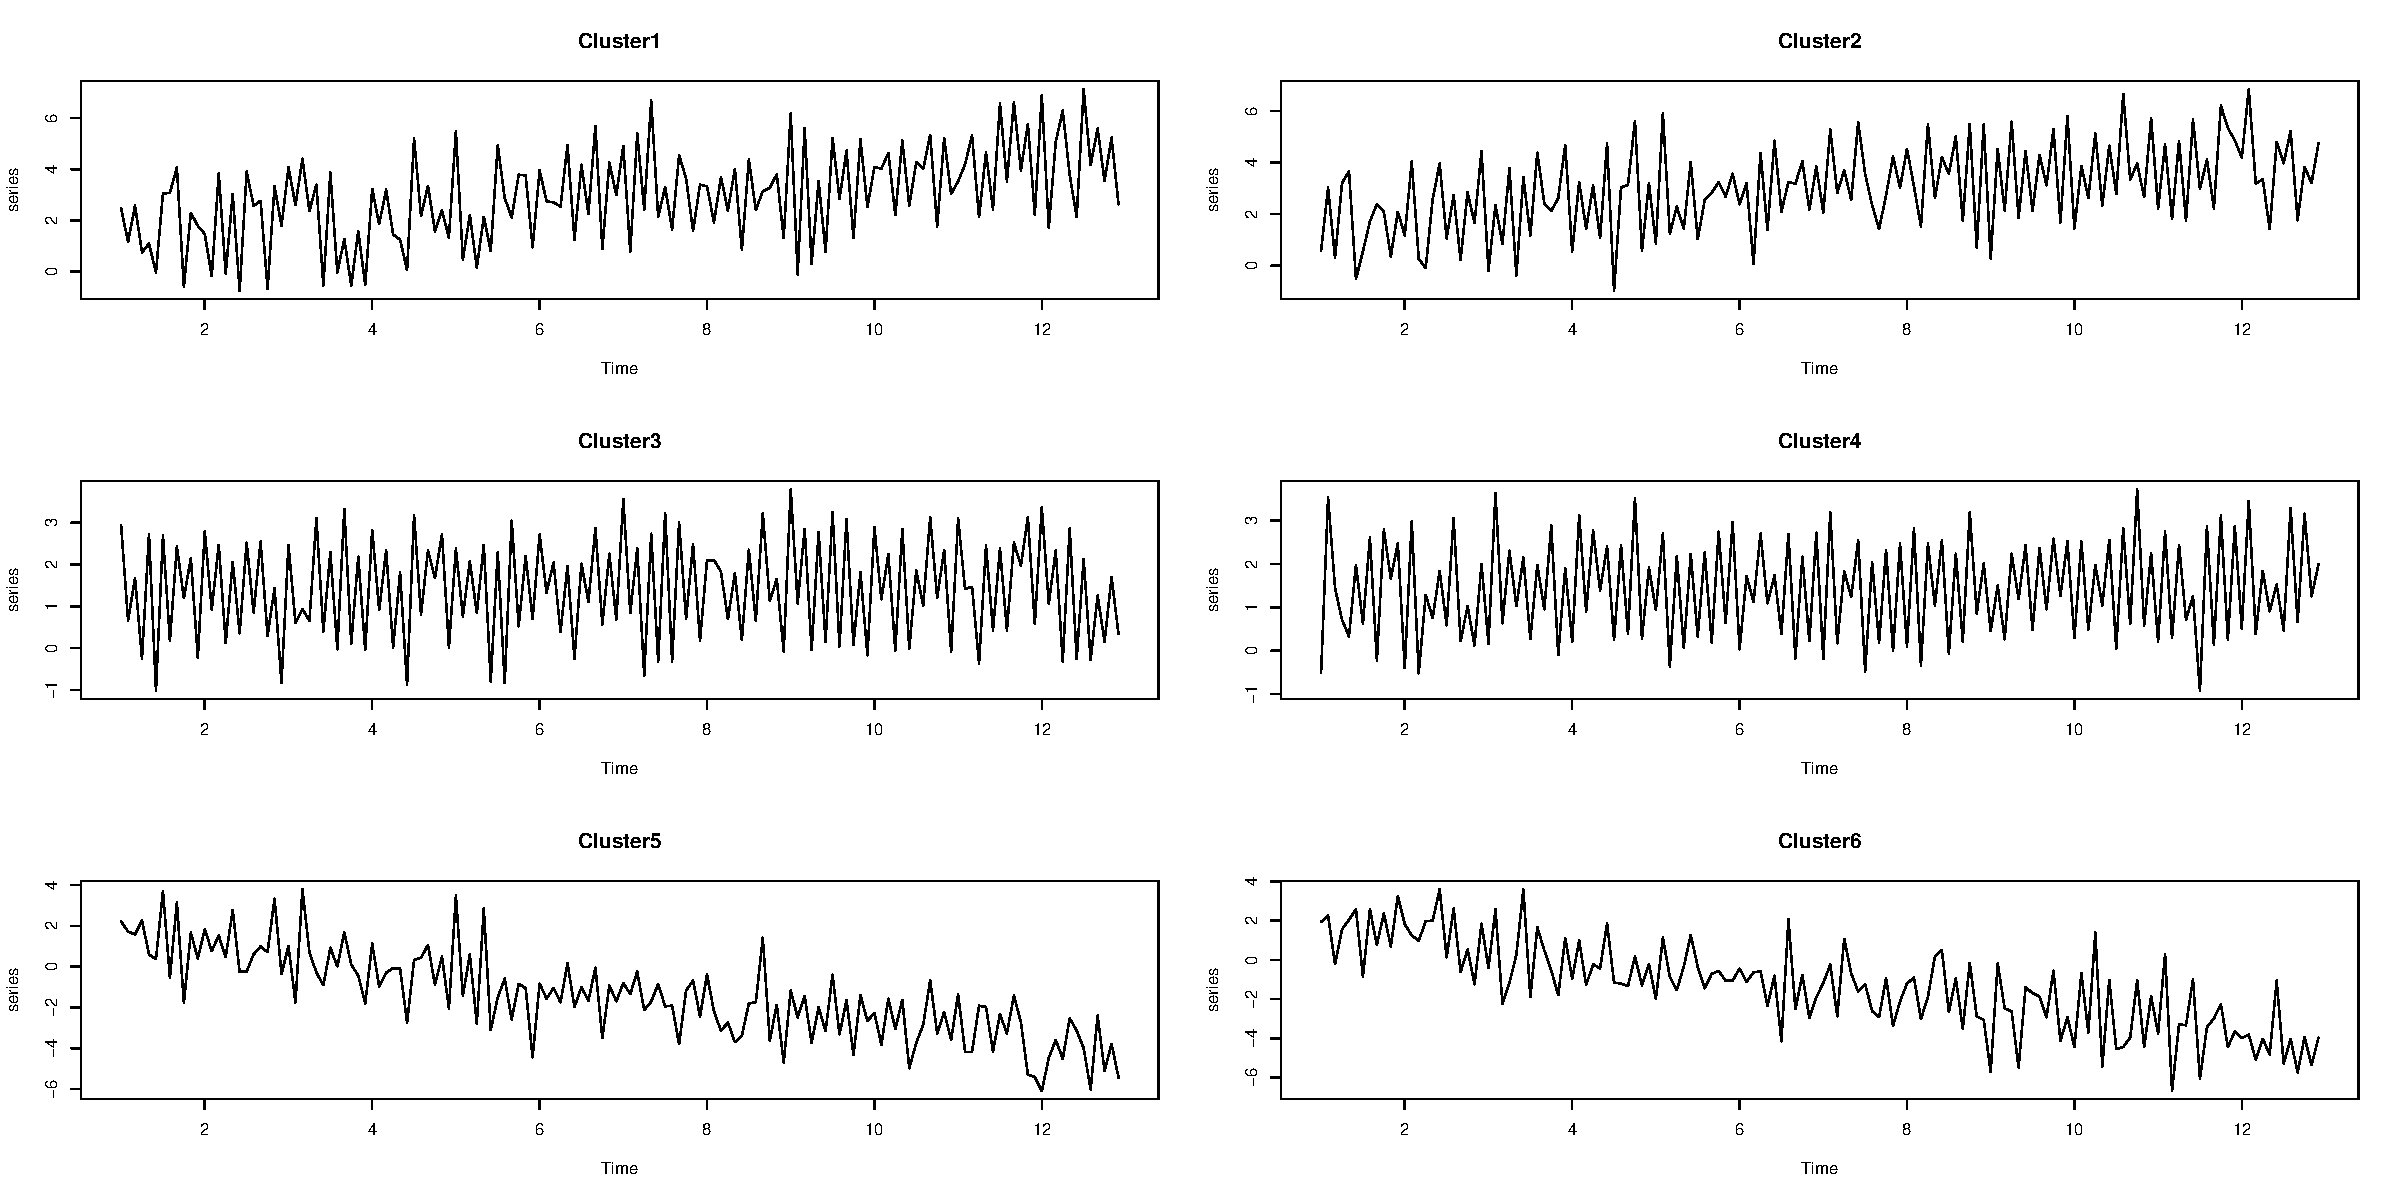
\includegraphics[width=\textwidth]{figures/simu_example.pdf}
\caption{\label{fig:simu_emps}Example time series for each cluster in the simulation experiments.}
\end{figure}

\begin{figure}
    \centering
    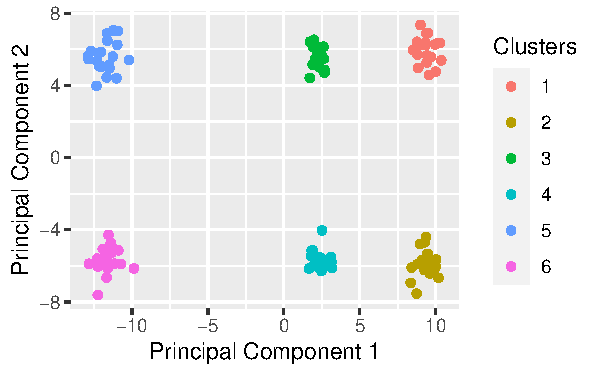
\includegraphics[width=0.6\textwidth]{figures/simu_pca.pdf}
    \caption{\label{fig:simu_pca}Visualisation of the generated time series in the simulation experiments.}
\end{figure}


\subsubsection*{Hierarchies construction}

There are a total of $120$ bottom series and $1$ total series in the hierarchy, referred to as ``C0''. Additionally, we consider $4$ clustering approaches and $2$ forecast combination approaches. ``C1'' creates $6$ middle-level series according to the designed correct clusters. We merge clusters with the same trend pattern, resulting in $3$ clusters in the middle level, denoted by ``C2''. Similarly, we construct ``C3'' and ``C4'' based on the presence of the trend term and seasonal peak positions, resulting in $2$ and $3$ middle-level series, respectively. ``A1'' combines reconciled forecasts obtained from all four clustering approaches (``C1'' to ``C4'') using equal weights. By shuffling the bottom-level series within the hierarchy ``C1'', we can randomly generate different hierarchies with identical structure. ``A2'' combines reconciled forecasts from $10$ randomly constructed hierarchies using equal weights.

\subsubsection*{Forecasting}

We construct two scenarios by considering different base forecasting models. In the first scenario, exponential smoothing (ETS) is used to generate base forecasts for all time series in hierarchies. This simulates a situation where the time series themselves are inputs to the clustering algorithms.
In the second scenario, we use historic mean to generate base forecasts for bottom-level series and ETS for other time series in hierarchies, which simulates the case where in-sample errors are inputs to the clustering algorithms. We refer to these scenarios as ``clustering by time series'' and ``clustering by error'', respectively. To reconcile the base forecasts, we employ the minimum trace method with the shrinkage estimator (\citealp{wickramasuriyaOptimalForecastReconciliation2019}). The shrinkage estimator is effective at capturing the dependence structure within the forecast errors and has demonstrated superior perofrmance in various applications. For each series, we generate $144$ observations, and the last $12$ observations are reserved for evaluation purpose.


\subsection{Evaluation}
\label{sec:simu_eval}

The purpose of constructing middle-level series is to improve the forecast performance of the total-level and bottom-level series by leveraging the strength of these new series.
Therefore, we only evaluate the reconciled forecasts at total level and bottom level. 
To assess the accuracy of single time series, we use root mean squared error (RMSE) as our metric. 
The simulation is repeated $500$ times, resulting in a total of $500\times 121$ RMSEs for each approach. 
Multiple comparisons with the best (MCB) test is then applied to compute the average ranks of the $7$ approaches along with base forecasts and to determine whether the performance differences are statistically different (\citealp{koningM3CompetitionStatistical2005}).


\subsection{Results}
\label{sec:simu_res}

Figure~\ref{fig:simu_mcb} displays the MCB test results for the two scenarios. 
In both scenarios, most approaches perform better than the base forecasts and the original two-level hierarchy ``C0''. This suggests that constructing middle-level series generally improves forecast reconciliation performance.
In the ``clustering by time series'' scenario, the correct cluster ``C1'' ranks $4$th, indicates that optimal clusters do not guarantee optimal forecast reconciliation performance. 
On the other hand, ``C1'' ranks $1$st in the ``clustering by error'' scenarios. This highlights the importance of carefully selecting time series representations when constructing new middle levels using clustering algorithms.
The simple average of $10$ random hierarchies ranks $1$st in the first scenario and the simple average of $4$ clustering hierarchies ranks $3$rd in both scenarios, indicating the importance of forecast combination.


\begin{figure}
    \centering
    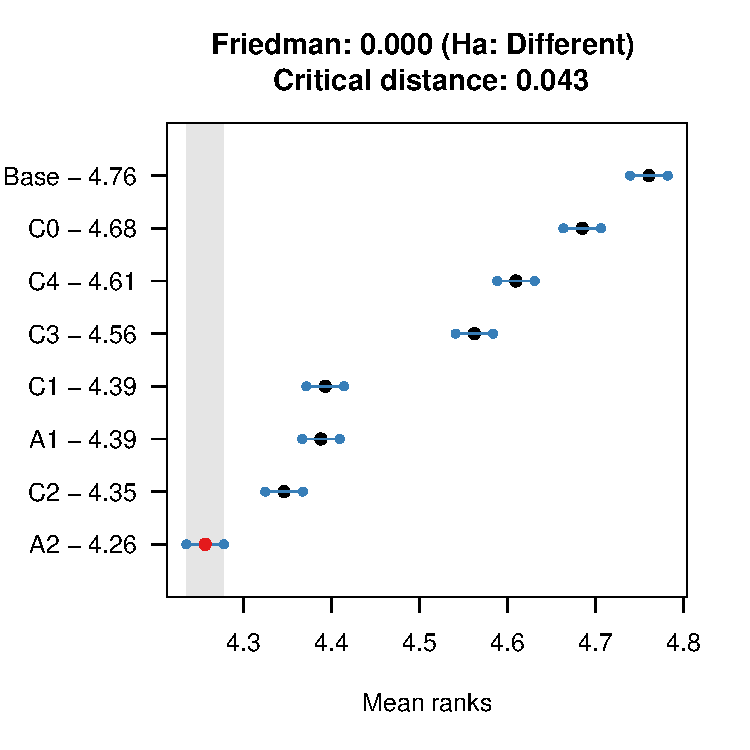
\includegraphics[width=0.45\textwidth]{figures/simu_mcb1.pdf}
    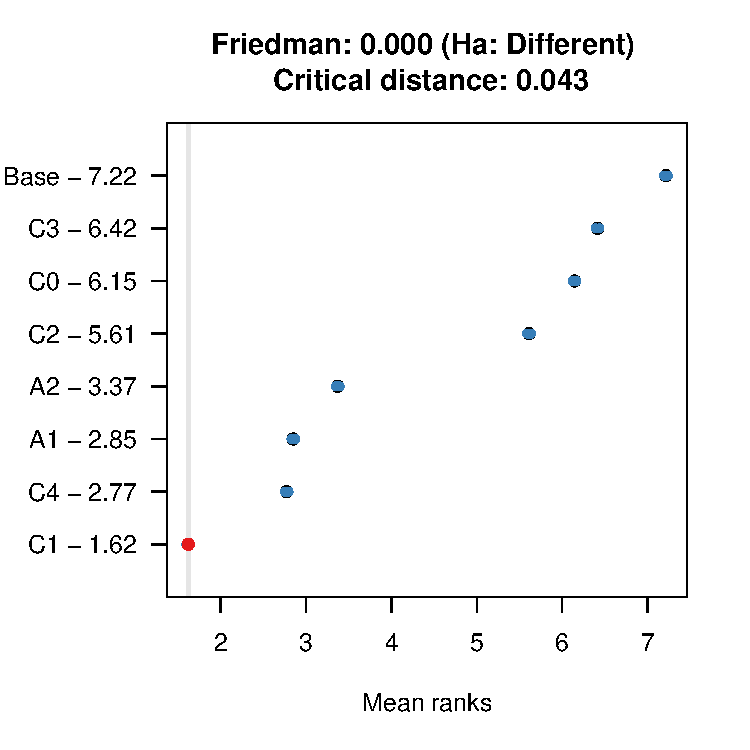
\includegraphics[width=0.45\textwidth]{figures/simu_mcb2.pdf}
    \caption{\label{fig:simu_mcb}Average ranks and 95\% confidence intervals based on the MCB Test for the $8$ approaches in the two scenarios of the simulation experiments. Left panel displays test results for the ``clustering by time series'' scenario and right panel displays test results for the ``clustering by error'' scenario.}
\end{figure}

\section{Empirical studies}

\subsection{Datasets}

We analyse two datasets in our empirical studies. The first dataset is the monthly Australian domestic tourism dataset, which provides visitor nights numbers from 1998 to 2016. The tourism demand of Australia is geographically disaggregated into $7$ states and territories, further divided into $27$ zones and $76$ regions. Additionally, each geographical series is divided by four travel purposes (\citealp{wickramasuriyaOptimalForecastReconciliation2019}). This dataset totally contains $555$ time series with $304$ at the bottom level.

The second dataset focuses on causes of death in the U.S., using the ICD 10 coding system. We obtain monthly cause-specific death counts from the Center for Disease Control and Prevention (CDC) for the period between 1999 and 2019. The coding system forms an unbalanced hierarchy with $137$ time series, out of which $113$ time series are in the bottom level. To consolidate data with suppressed values, we combine causes that share a parent cause and calculate their death counts by subtracting death counts of sibling causes from death counts of their parent cause. The final dataset includes $120$ time series with $98$ in the bottom level.

\subsection{Experiment design}

We focus on the performance of total-level series and bottom-level series, disregarding the multiple middle levels in the original hierarchies known as "natural hierarchies". The natural hierarchy is considered one way to construct middle-level series, similar to hierarchies created through clustering. However, we demonstrate that for the purpose of forecast performance, the natural hierarchy may not be the most effective hierarchical structure.

To construct middle levels using clustering, we combine four time series representations with two distance measures and two clustering algorithms. This results in twelve different construction approaches listed in Table~\ref{tab:emp_method}.


\begin{table}
\caption{\label{tab:emp_method} Hierarchy construction approaches used in empirical studies.}
\centering
\resizebox{\textwidth}{!}{
\begin{tabular}{ccccc}
    \toprule
    Approaches & Representation & Dimension reduction & Distance measure & Clustering algorithms  \\
    TS-MED & Time series & Yes & Euclidean & k-Medoids \\
    ER-MED & In-sample error & Yes & Euclidean & k-Medoids \\
    TSF-ME & Time series features & Yes & Euclidean & k-Medoids \\
    ERF-ME & In-sample error features & Yes & Euclidean & k-Medoids \\
    TS-HC & Time series & Yes & Euclidean & hierarchical clustering  \\ 
    ER-HC & In-sample error & Yes & Euclidean & hierarchical clustering  \\ 
    TSF-HC & Time series features & Yes & Euclidean & hierarchical clustering  \\ 
    ERF-HC & In-sample error features & Yes & Euclidean & hierarchical clustering  \\
    TS-MED-DTW & Time series & No & DTW & k-Medoids \\
    TS-HC-DTW & In-sample error & No & DTW & hierarchical clustering \\
    ER-MED-DTW & Time series & No & DTW & k-Medoids \\
    ER-HC-DTW & In-sample error & No & DTW & hierarchical clustering 
     \\\bottomrule
\end{tabular}}
\end{table}

Additionally, we consider three forecast combination approaches. In the first approach, we create one middle level with $15$ time series by randomly assigning bottom-level series as their children. We ensure that all the middle-level series have approximately an equal number of children. The choice of having $15$ middle-level series is arbitrary with the goal of creating a moderate number of groups, each containing a moderate number of series.
We repeat this process to create $50$ such hierarchies and combine their reconciled forecasts using equal weights. This approach is referred to as ``FC-R''.
In the second approach, we create $10$ new hierarchies by randomly shuffling the positions of bottom-level series in the natural hierarchy and combine their reconciled forecasts using equal weights. This approach is denoted by ``FC-N''. The third approach, labelled by ``FC-C'', involves equally-weighted combining the reconciled forecasts obtained from the $12$ hierarchies shown in Table~\ref{tab:emp_method}.

The time series features used in this experiment are calculated using the \texttt{tsfeatures} package (\citealp{tsfeatures}) for R. After filtering out the features that are constant across all series, $56$ features are reserved. The complete list of these feature can be found in Appendix. The k-Medoids and hierarchical clustering algorithms are implemented using the \texttt{cluster}(\citealp{cluster}) package for R. The base forecasts are generated using the automatic ETS models, which are then reconciled using the minimum trace method with shrinkage estimator.

We employ the rolling window strategy to evaluate the performance of different approaches for both datasets. We start with $96$ observations and fit the base forecasting models using the available data. Then we calculate time series representations and construct new hierarchies by clustering or randomness, and then forecast $12$ steps ahead. After that, the training set is increased by one observation and new forecasts are obtained. The procedure is repeated until the last $12$ observations are used for evaluation. Finally, we can obtain $121$ $12$-step-ahead forecasts for the tourism dataset and $144$ $12$-step-ahead forecasts for the mortality dataset. We compare the forecast performance of the $15$ approaches as well as the natural hierarchy, two-level hierarchy and base forecasts for both total-level and bottom-level series. 

\subsection{Results}

Same as the evaluation measure described in Section~\ref{sec:simu_eval}, we combine the forecasts of total-level and bottom-level series across all evaluation windows and conduct the MCB test. The test results for the tourism dataset and mortality dataset are shown in Figure~\ref{fig:tourism_mcb} and Figure~\ref{fig:mortality_mcb}, respectively.

Most hierarchy construction approaches outperform both base forecasts and the two-level hierarchy, except for three approaches on the mortality dataset. For both datasets, the simple average of randomised natural hierarchies (``FC-N'') performs better than both natural hierarchy and all clustering-based hierarchies. Additionally, the simple average of $12$ clustering-based hierarchies (``FC-C'') significantly outperforms all other approaches. These results indicate that using a clustering-based hierarchy can improve forecast performance. However, forecast combination is even more beneficial, as evidenced by the high ranking of ``FC-N'' and ``FC-R''.

\begin{figure}
    \centering
    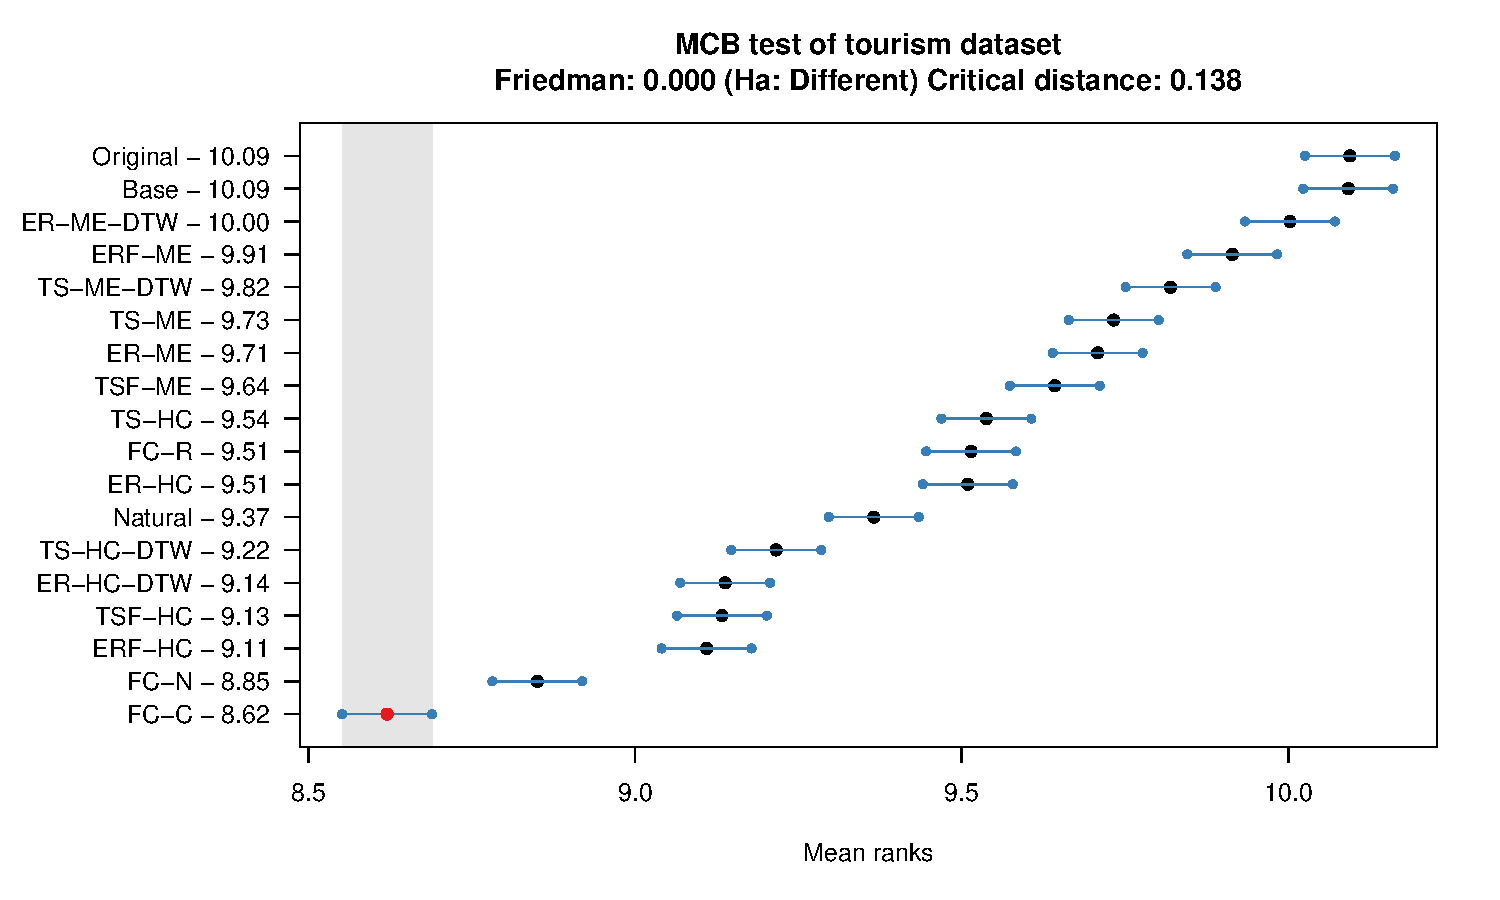
\includegraphics[width=\textwidth]{figures/tourism_mcb.pdf}
    \caption{\label{fig:tourism_mcb}Average ranks and 95\% confidence intervals based on the MCB Test for the $18$ approaches on the tourism dataset.}
\end{figure}

\begin{figure}
    \centering
    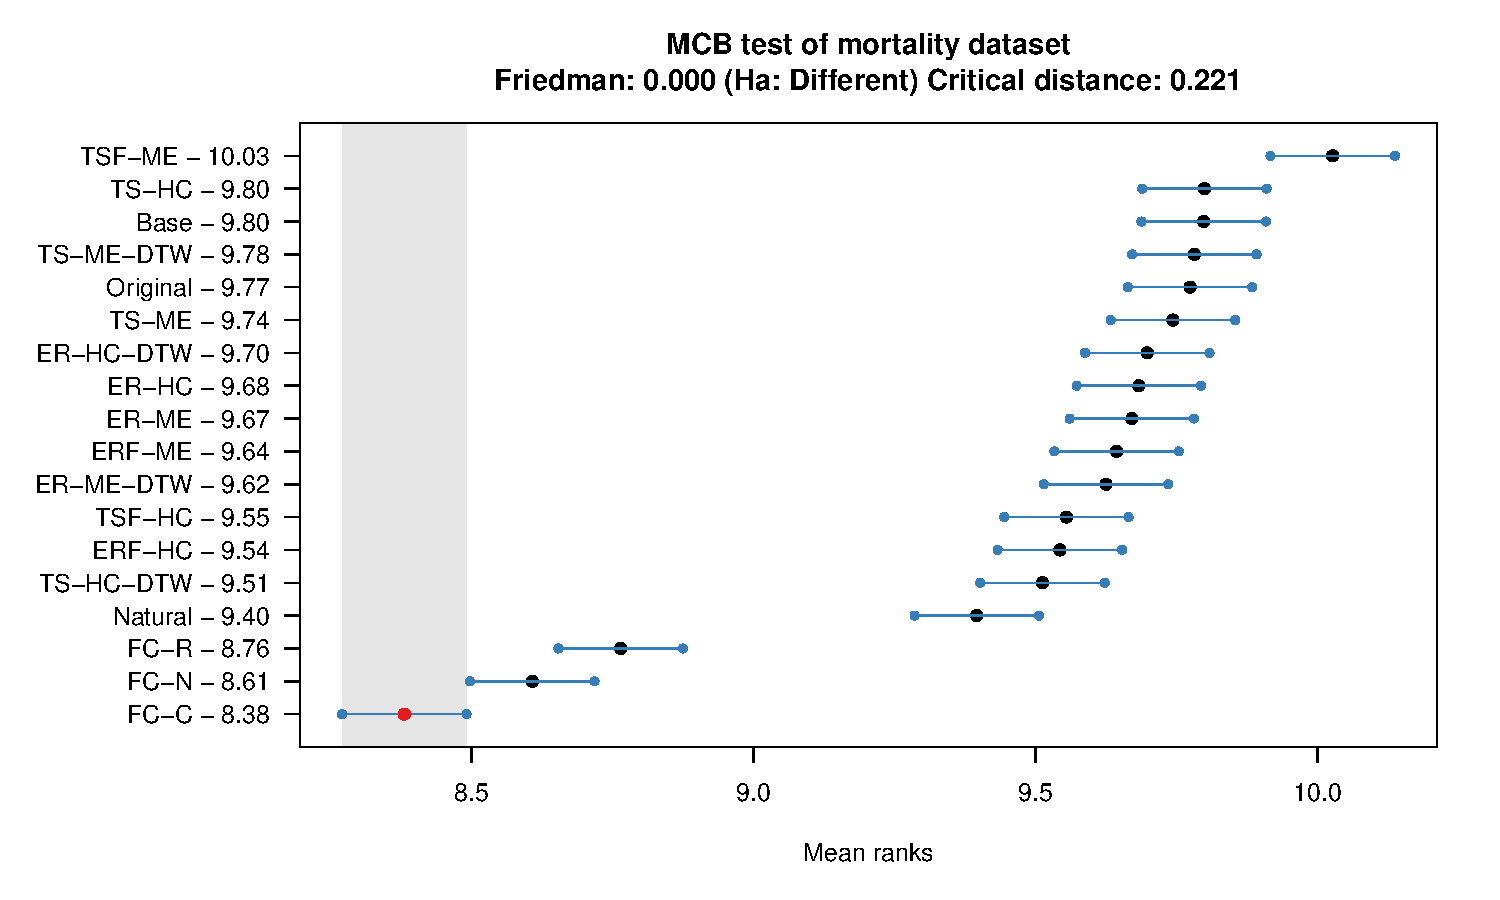
\includegraphics[width=\textwidth]{figures/mortality_mcb.pdf}
    \caption{\label{fig:mortality_mcb}Average ranks and 95\% confidence intervals based on the MCB Test for the $18$ approaches on the mortality dataset.}
\end{figure}

The approach based on hierarchical clustering outperforms the approach based on k-Medoids on the tourism dataset when using the same representation and distance metric, e.g., ``TSF-HC'' significantly ourperforms ``TSF-ME''. However, this is not consistently observed for every combination of representation and distance metric on the mortality dataset. We believe this discrepancy is due to different time series patterns at the bottom level of these two datasets.
In the case of the mortality dataset, we combine rare causes of death that have suppressed values and record death counts at a national level. As a result, most series at the bottom level exhibit strong seasonality and trend. On the other hand, in the tourism dataset, the tourism demand is disaggregated for both travel purposes and geographical regions. This leads to numerous bottom-level series with high volatility and many zeros, making them more challenging to forecast.
Therefore, having a hierarchy with more middle-level series can be more advantageous for reconciliation in the tourism dataset compared to the mortality dataset. Additionally, we suspect that the inferior performance of ``FC-R'' on the tourism dataset may be partly attributed to an insufficient number of middle-level series.

In most cases, the in-sample error representation outperforms the time series representation when using the same distance metric and clustering algorithms. However, this performance difference is not as significant as what was observed in Section~\ref{sec:simu_res}. Intuitively, hierarchies constructed based on clustering in-sample error should be similar to random hierarchies when all base models are correctly specified. However, due to ubiquitous model misspecification in practice, vague patterns emerge in the in-sample error, which leads to contradictory results.


\subsubsection*{Effect of number of random hierarchies}

In our previous experiments, we set the number of random hierarchies in ``FC-R'' and ``FC-N'' to $10$ for fair comparisons with ``FC-C''. However, we believe that increasing the number of random hierarchies could further enhance performance. In this subsection, we explore the effects of using 20 and 50 random hierarchies, referred to as ``FC-N-20'', ``FC-N-50'', ``FC-R-20'', and ``FC-R-50''. We compare these variations with ``FC-R'', ``FC-C'', and ``FC-N'' using the same evaluation procedure described earlier. The results from the MCB test are presented in Figure~\ref{fig:number_mcb}, where the left panel shows results on the tourism dataset and the right panel displays results on the mortality dataset.

Generally, we observe that forecast performance improves as the number of random hierarchies increases, except for ``FC-N-20'' and ``FC-N'' on the mortality dataset. Surprisingly, on the tourism dataset, ``FC-N-50'' performs slightly better than ``FC-C''. It is important to note that employing more random hierarchies comes at a cost of increased computational resources. Therefore, one must carefully consider trade-offs between efficiency and performance when making decisions.

\begin{figure}
\centering
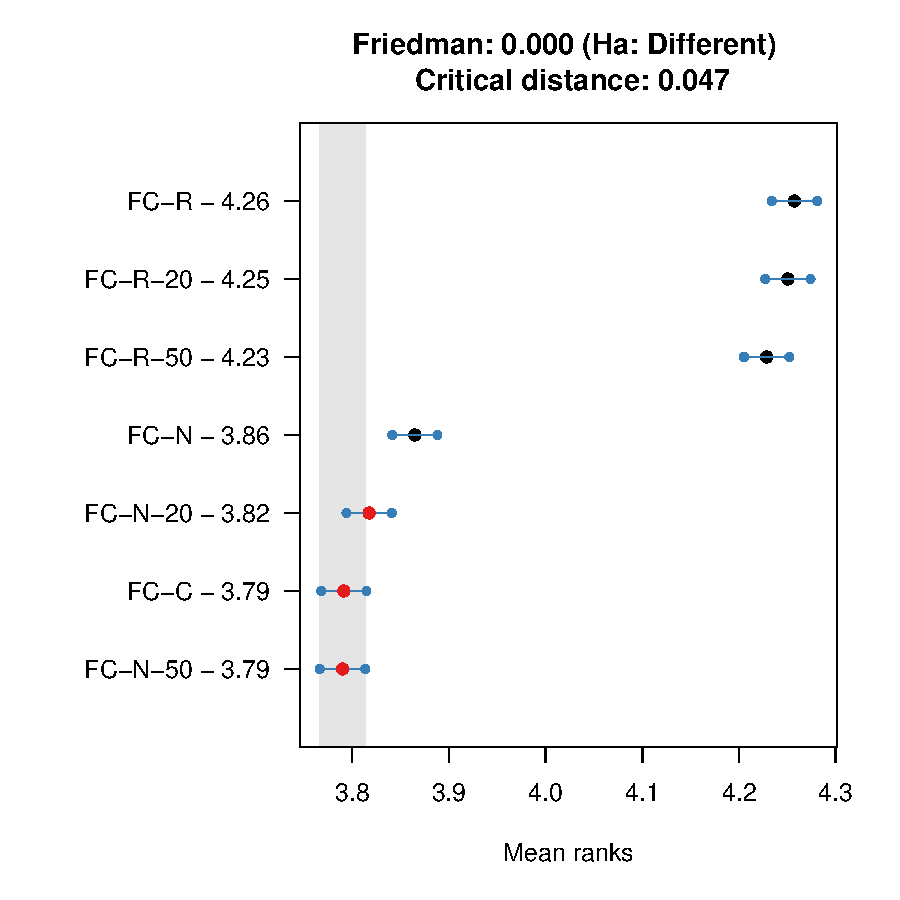
\includegraphics[width=0.45\textwidth]{figures/tourism_number_mcb.pdf}
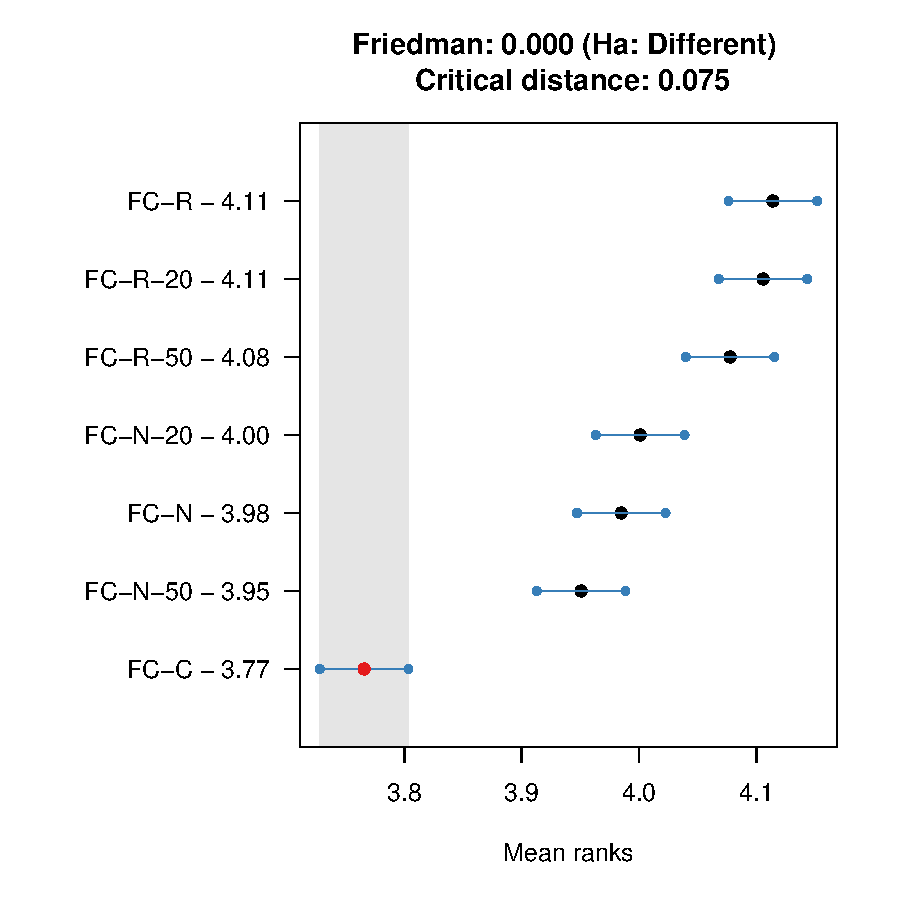
\includegraphics[width=0.45\textwidth]{figures/mortality_number_mcb.pdf}
\caption{\label{fig:number_mcb}Average ranks and 95\% confidence intervals based on the MCB Test of different number of random hierarchies on two datasets. Left and right panels display test results on tourism dataset and mortality dataset, respectively.}
\end{figure}

\section{Conclusion}
\label{sec:conclusion}


\section*{Acknowledgements}



\begingroup
\setstretch{1.15}
\bibliographystyle{agsm}
\bibliography{references.bib}
\endgroup



\end{document}